\documentclass[11pt]{article}
\usepackage[margin=1in]{geometry}
\usepackage{amsmath,amssymb,graphicx,float,verbatim,mathpazo}
\usepackage[colorlinks=true]{hyperref}
\setlength{\parindent}{0pt}\setlength{\parskip}{0.6\baselineskip}\emergencystretch=2em
\newcommand\xstart{+0.890}
\newcommand\Kerr{1.3e-04}
\newcommand\Nmin{0.99940}
\newcommand\Emin{1.0179}
\newcommand\Emax{1.0214}
\newcommand\Eex{1.0211}
\newcommand\NormI{9.99\times10^{-1}}
\newcommand\NormII{1.15\times10^{258}}
\newcommand\NormIII{4.10\times10^{51}}
\newcommand\nmaxA{369}
\newcommand\nmaxB{741}
   % numbers written by assignment1.ipynb

\title{PHYS 142/242 --- Assignment 1\\\large Harmonic Oscillator Path Integral}
\author{}\date{}

\begin{document}
\maketitle
\vspace{-2.5em}
\begin{center}\Large $x_\mathrm{start} = \xstart$\end{center}

All code is in \texttt{assignment1.ipynb} (Python/NumPy); running it top to bottom produces every figure,
the animation \texttt{animation.gif}, the autograder file \texttt{results.json}, and the numbers quoted below.
Units $m=\omega=\hbar=1$, grid $x_i\in[-4,4]$ with $N_D=600$ ($\Delta x = 8/600$), $\epsilon=T_0/128$, $\alpha=2$.
One time step is $\psi_{n+1} = \Delta x\,\mathcal K_\epsilon\,\psi_n$, where
$(\mathcal K_\epsilon)_{ba} = \mathcal K(x_b,\epsilon;x_a,0)$ is the exact propagator evaluated on the grid.

\section*{Problem A: $\mathcal K_{8\epsilon}$}
$\mathcal K_{8\epsilon} = (\Delta x)^7 \mathcal K_\epsilon^8$ (computed with \texttt{np.linalg.matrix\_power}); \texttt{print(K\_8eps)} gives
{\footnotesize\verbatiminput{figs/K8eps.txt}}
The matrix is complex symmetric, and also symmetric under $(x_a,x_b)\to(-x_a,-x_b)$, as the analytic formula requires.
As a check, $\Delta x\,\mathcal K_{8\epsilon}\psi_0$ agrees with a single application of the exact propagator
$\mathcal K(\cdot,T_0/16;\cdot,0)$ to $\psi_0$ to within $\Kerr$ (max.\ abs.\ difference).
Individual matrix elements, however, differ from the exact kernel everywhere (by $\sim$10--20\% in the interior and $O(1)$ near the edges).
The exact kernel is a rapidly oscillating distribution: the grid cannot represent its high-wavenumber part, and the intermediate
integrals are cut off at $\pm4$. Only the \emph{action} of $\mathcal K_{8\epsilon}$ on smooth, localized states converges, and that is all the evolution needs.

\section*{Problem B: $\langle x\rangle(t)$}
$\langle x\rangle = \Delta x\sum_i x_i |\psi_i|^2$. The state is not renormalized; its norm $\mathcal N=\Delta x\sum_i|\psi_i|^2$ stays in $[\Nmin, 1]$.
The numerical result lies on top of the classical trajectory $x_\mathrm{start}\cos t$ (Ehrenfest's theorem).
\begin{figure}[H]\centering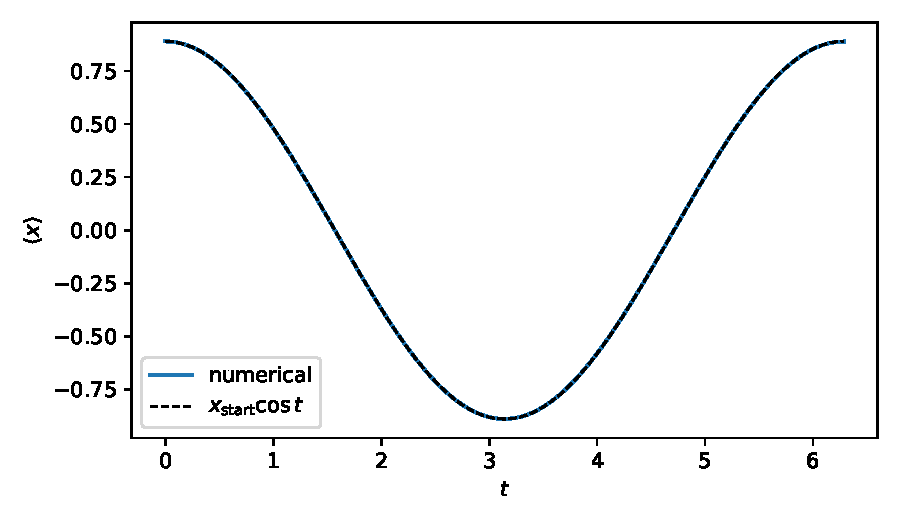
\includegraphics[width=0.65\textwidth]{figs/mean_x.pdf}
\caption{Mean position over one period; dashed line is $x_\mathrm{start}\cos t$.}\end{figure}

\section*{Problem C: $\langle E\rangle$, $\langle K\rangle$, $\langle V\rangle$}
$\langle V\rangle = \Delta x\sum_i \tfrac12 x_i^2|\psi_i|^2$ and
$\langle K\rangle = \tfrac12\Delta x\sum_i |\partial_x\psi|_i^2$, with $\partial_x\psi$ from central differences (\texttt{np.gradient}).
$\langle E\rangle$ is conserved: it stays in $[\Emin,\Emax]$, compared with the exact value
$\langle E\rangle = \tfrac14(\alpha+\alpha^{-1}) + \tfrac12 x_\mathrm{start}^2 = \Eex$
The small downward drift comes mainly from cutting the $x$ integrals off at the box edge $\pm4$, which makes the one-step matrix slightly non-unitary.
It shows up as the same size error in $\langle V\rangle$, which uses no derivative, and it disappears on a larger box with the same $\Delta x$.
The finite-difference derivative contributes only $\sim10^{-4}$. The norm loss ($\mathcal N\geq\Nmin$, another symptom of the same truncation) lowers $\langle E\rangle$ by at most $0.06\%$, since the state is not renormalized.
$\langle K\rangle$ and $\langle V\rangle$ exchange energy at frequency $2\omega$. Analytically
\[\langle V\rangle = \tfrac12x_\mathrm{start}^2\cos^2t + \tfrac14\left(\alpha^{-1}\cos^2t+\alpha\sin^2t\right),\qquad \langle K\rangle=\langle E\rangle-\langle V\rangle.\]
Two terms oscillate here. The first, $\tfrac12x_\mathrm{start}^2\cos^2t$, is the classical motion of the centre and is present even for a coherent state ($\alpha=1$).
The second comes from the width ``breathing'', because $\alpha=2$ makes the packet narrower than the ground state.
They have opposite phase: $\langle V\rangle=\text{const}+\big[x_\mathrm{start}^2/4-(\alpha-\alpha^{-1})/8\big]\cos2t$.
For $x_\mathrm{start}=\xstart$ they nearly cancel, which is why the $\langle K\rangle$ and $\langle V\rangle$ curves vary so little.
\begin{figure}[H]\centering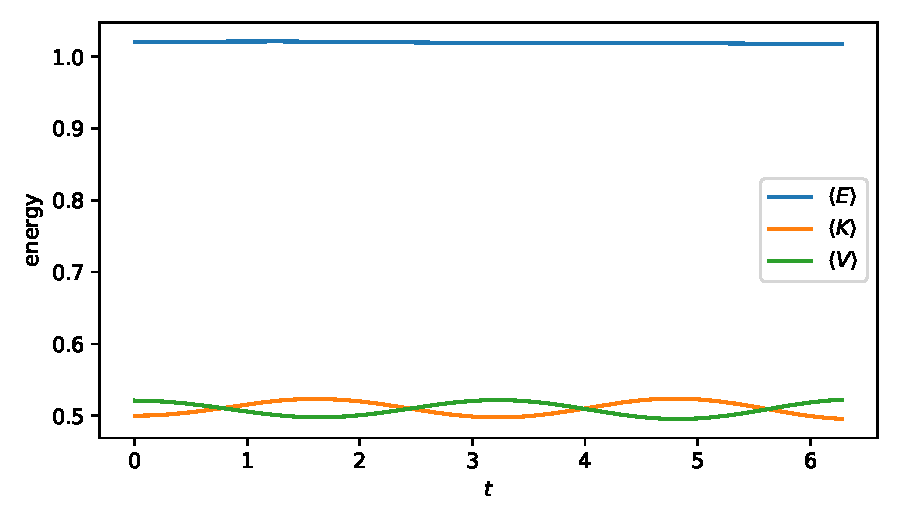
\includegraphics[width=0.65\textwidth]{figs/energy.pdf}
\caption{Mean total, kinetic and potential energy over one period.}\end{figure}

\section*{Problem D: snapshots at $t=mT_0/16$}
The packet moves from $x_\mathrm{start}$ to $-x_\mathrm{start}$ in half a period.
It is narrowest (tallest) at $t=0$ and $T_0/2$ and widest at $t=T_0/4$, consistent with the width oscillation seen in Problem C.
\begin{figure}[H]\centering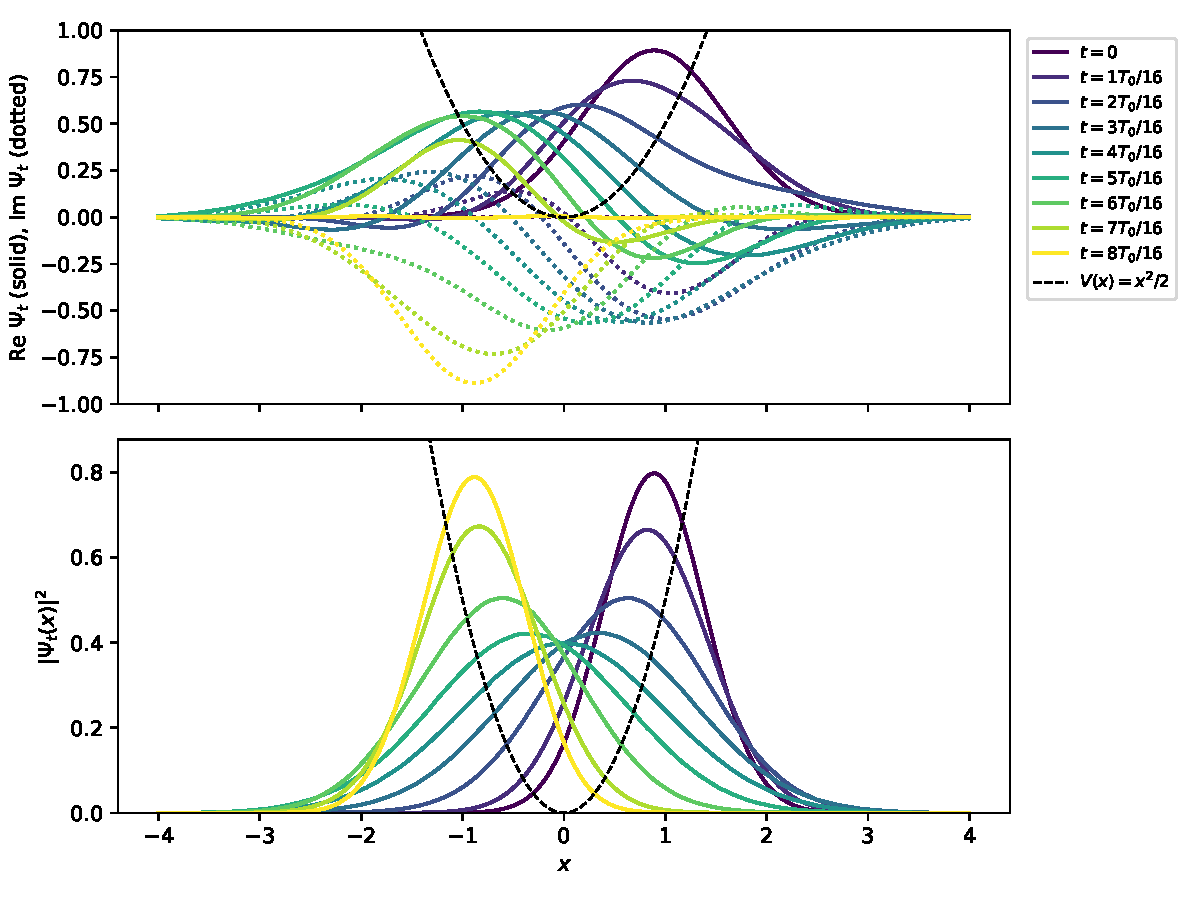
\includegraphics[width=0.8\textwidth]{figs/snapshots.pdf}
\caption{Top: amplitude $\mathrm{Re}\,\Psi_t$ (solid) and $\mathrm{Im}\,\Psi_t$ (dotted). Bottom: $P_t(x)=|\Psi_t(x)|^2$. Both at $t=mT_0/16$, $m=0,\dots,8$, with $V(x)=x^2/2$ superimposed.}\end{figure}

\section*{Problem E: animation}
\texttt{animation.gif} (submitted with the code) has 129 frames, one per step $\epsilon$ from $t=0$ to $T_0$.
It shows $|\Psi|^2$, $\mathrm{Re}\,\Psi$, $\mathrm{Im}\,\Psi$ and $V(x)$.
After one full period the state returns to $\Psi_0$ up to the global phase $e^{-i\pi}$, so $\mathrm{Re}\,\Psi$ is flipped in the last frame.

\section*{Problem F (bonus): norm without renormalization}
\textbf{Prediction.} The propagator is exact for any $\epsilon$, so the only error is replacing $\int dx_a$ by $\Delta x\sum_a$.
The phase of $\mathcal K_\epsilon(x_b,x_a)$ is $\phi=[(x_a^2+x_b^2)\cos\epsilon-2x_ax_b]/(2\sin\epsilon)$, so as a function of $x_a$ it oscillates with local wavenumber
\[
  k = \frac{\partial\phi}{\partial x_a} = \frac{x_a\cos\epsilon-x_b}{\sin\epsilon}\approx\frac{x_a-x_b}{\epsilon}.
\]
The integral $\int dx_a\,\mathcal K_\epsilon(x_b,x_a)\psi(x_a)$ is dominated by the stationary point $k=0$ ($x_a\approx x_b$), and elsewhere the fast oscillation cancels.
On a grid, however, $e^{ikx_a}$ and $e^{i(k-2\pi/\Delta x)x_a}$ are the same sequence.
So the sum $\Delta x\sum_a$ also sees spurious ``aliased'' stationary points wherever $|k|\Delta x = 2\pi$, i.e.\ at $|x_a-x_b|\approx 2\pi\epsilon/\Delta x$.
These give large, non-cancelling contributions.
They stay outside the box, whose full width is $8$, only if $2\pi\epsilon/\Delta x > 8$:
\[
  \epsilon > \epsilon_\mathrm{min} = \frac{4\Delta x}{\pi} = \frac{32}{\pi N_D}.
\]
This depends only on the grid and the box, not on the initial state.
For $N_D=600$, $\epsilon_\mathrm{min}\approx0.017\approx T_0/370$; for $N_D=150$, $\epsilon_\mathrm{min}\approx0.068\approx T_0/93$.
So I predicted (i) $\epsilon=T_0/16=0.39$ works, while (ii) $\epsilon=T_0/512=0.012$ and (iii) $\epsilon=T_0/128$ with $N_D=150$ both fail.

\textbf{Result.} After one period $\mathcal N(T_0) = \NormI$ for (i), $\NormII$ for (ii), and $\NormIII$ for (iii).
Cases (ii) and (iii) grow exponentially (straight lines on the log plot): when the kernel is undersampled, its aliased phase
no longer cancels, the discrete one-step matrix $\Delta x\,\mathcal K_\epsilon$ is no longer (close to) unitary and has eigenvalues with $|\lambda|>1$,
so the norm is multiplied by a roughly constant factor each step.
Counter-intuitively, the \emph{larger} step (i) is the stable one: a small $\epsilon$ makes $\mathcal K_\epsilon$ oscillate faster, not slower.
\begin{figure}[H]\centering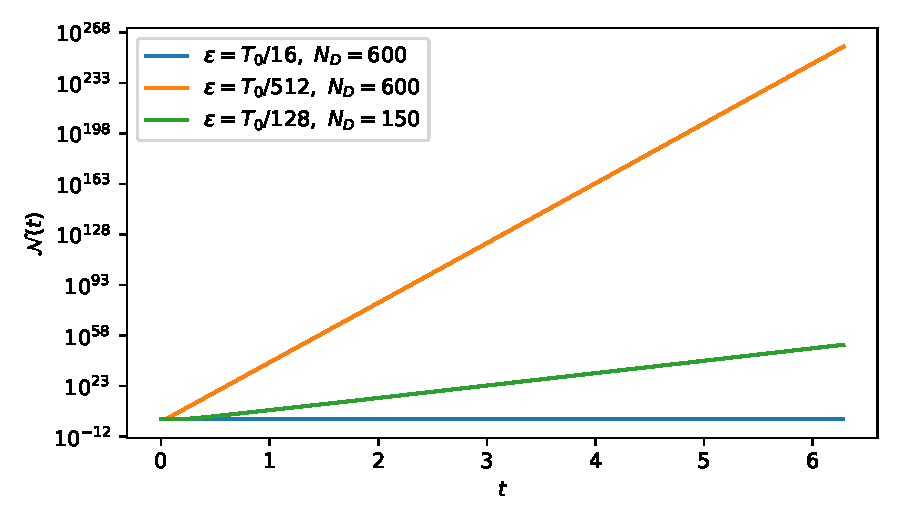
\includegraphics[width=0.65\textwidth]{figs/norm.pdf}
\caption{$\mathcal N(t)$ over one period for the three cases (log scale).}\end{figure}

\textbf{Smallest time step.} Bisecting on $n=T_0/\epsilon$ (stable = $\mathcal N$ stays within 1\% of 1 over one period) gives
$\epsilon_\mathrm{min} = T_0/\nmaxA \approx 0.0170$ for $N_D=600$, and $T_0/\nmaxB \approx 0.0085$ for $N_D=1200$,
in agreement with the estimate $32/(\pi N_D)$.
The box-size dependence is confirmed too: at the same $\Delta x$ on $[-8,8]$ the threshold doubles to $T_0/187$, and it is unchanged for $x_\mathrm{start}=0$.
Doubling $N_D$ halves $\Delta x$ and therefore halves the smallest usable time step: $\epsilon_\mathrm{min}\propto\Delta x\propto 1/N_D$.

\end{document}
